\documentclass{fisatprojectfinal}
\title{Pose Estimation Using Deep Learning}
\team{Aman K. Shihab \\ Aneeta Shajan}
\author{Aman K. Shihab}
\regno{FIT19CS015}
\begin{document}
\maketitle
\makecert

\newpage
\pagenumbering{roman}
\setcounter{page}{1}
\newgeometry{top=4cm,bottom=0.1cm}
\thispagestyle{plain}
\renewcommand\abstractname{ABSTRACT}
\begin{abstract}
\vspace{5cm}
Single-person human pose estimation facilitates markerless movement analysis in sports, as well as in clinical applications.
Still, state-of-the-art models for human pose estimation generally do not meet the requirements of real-life applications.
The proliferation of deep learning techniques has resulted in the development of many advanced approaches. However,
with the progresses in the field, more complex and inefficient models have also been introduced, which have caused
tremendous increases in computational demands. To cope with these complexity and inefficiency challenges, we propose
a novel convolutional neural network architecture, called EfficientPose, which exploits recently proposed EfficientNets
in order to deliver efficient and scalable single-person pose estimation. EfficientPose is a family of models harnessing
an effective multi-scale feature extractor and computationally efficient detection blocks using mobile inverted bottleneck
convolutions, while at the same time ensuring that the precision of the pose configurations is still improved. Due to its low
complexity and efficiency, EfficientPose enables real-world applications on edge devices by limiting the memory footprint
and computational cost. The results from our experiments, using the challenging MPII single-person benchmark, show that
the proposed EfficientPose models substantially outperform the widely-used OpenPose model both in terms of accuracy and
computational efficiency. In particular, our top-performing model achieves state-of-the-art accuracy on single-person MPII,
with low-complexity ConvNets.
\end{abstract}



\newpage
\renewcommand\abstractname{Contribution by Author}
\thispagestyle{plain}
\begin{abstract}
\vspace{5cm}
Author Contribution  Goes Here
\vspace{1cm}
\begin{flushright}
Student Name
\end{flushright}
\end{abstract}

\newpage
\renewcommand\abstractname{ACKNOWLEDGEMENT}
\thispagestyle{plain}
\begin{abstract}
\vspace{5cm}
Your Acknowledgement Goes Here
\vspace{1cm}
\begin{flushright}
Student 1
\end{flushright}
\end{abstract}
\newpage

\restoregeometry
\tableofcontents
\thispagestyle{plain}
\newpage

\cleardoublepage
\addcontentsline{toc}{chapter}{\listfigurename}
\listoffigures
\newpage

\cleardoublepage
\addcontentsline{toc}{chapter}{\listtablename}
\listoftables
\newpage



\chapter{Introduction}
\pagenumbering{arabic}
\setcounter{page}{1}
\renewcommand{\baselinestretch}{1.50}
\section{Overview}
Single-person human pose estimation (HPE) refers to the
computer vision task of localizing human skeletal keypoints
of a person from an image or video frames. Single-
person HPE has many real-world applications, ranging from
outdoor activity recognition and computer animation to clinical assessments of motor repertoire and skill practice
among professional athletes. The proliferation of deep
convolutional neural networks (ConvNets) has advanced
HPE and further widen its application areas. ConvNet-based
HPE with its increasingly complex network structures,
combined with transfer learning, is a very challenging task.
However, the availability of high-performing ImageNet
backbones, together with large tailor-made datasets, such
as MPII for 2D pose estimation, has facilitated the
development of new improved methods to address the
challenges.
\begin{figure}[h!]
\begin{center}
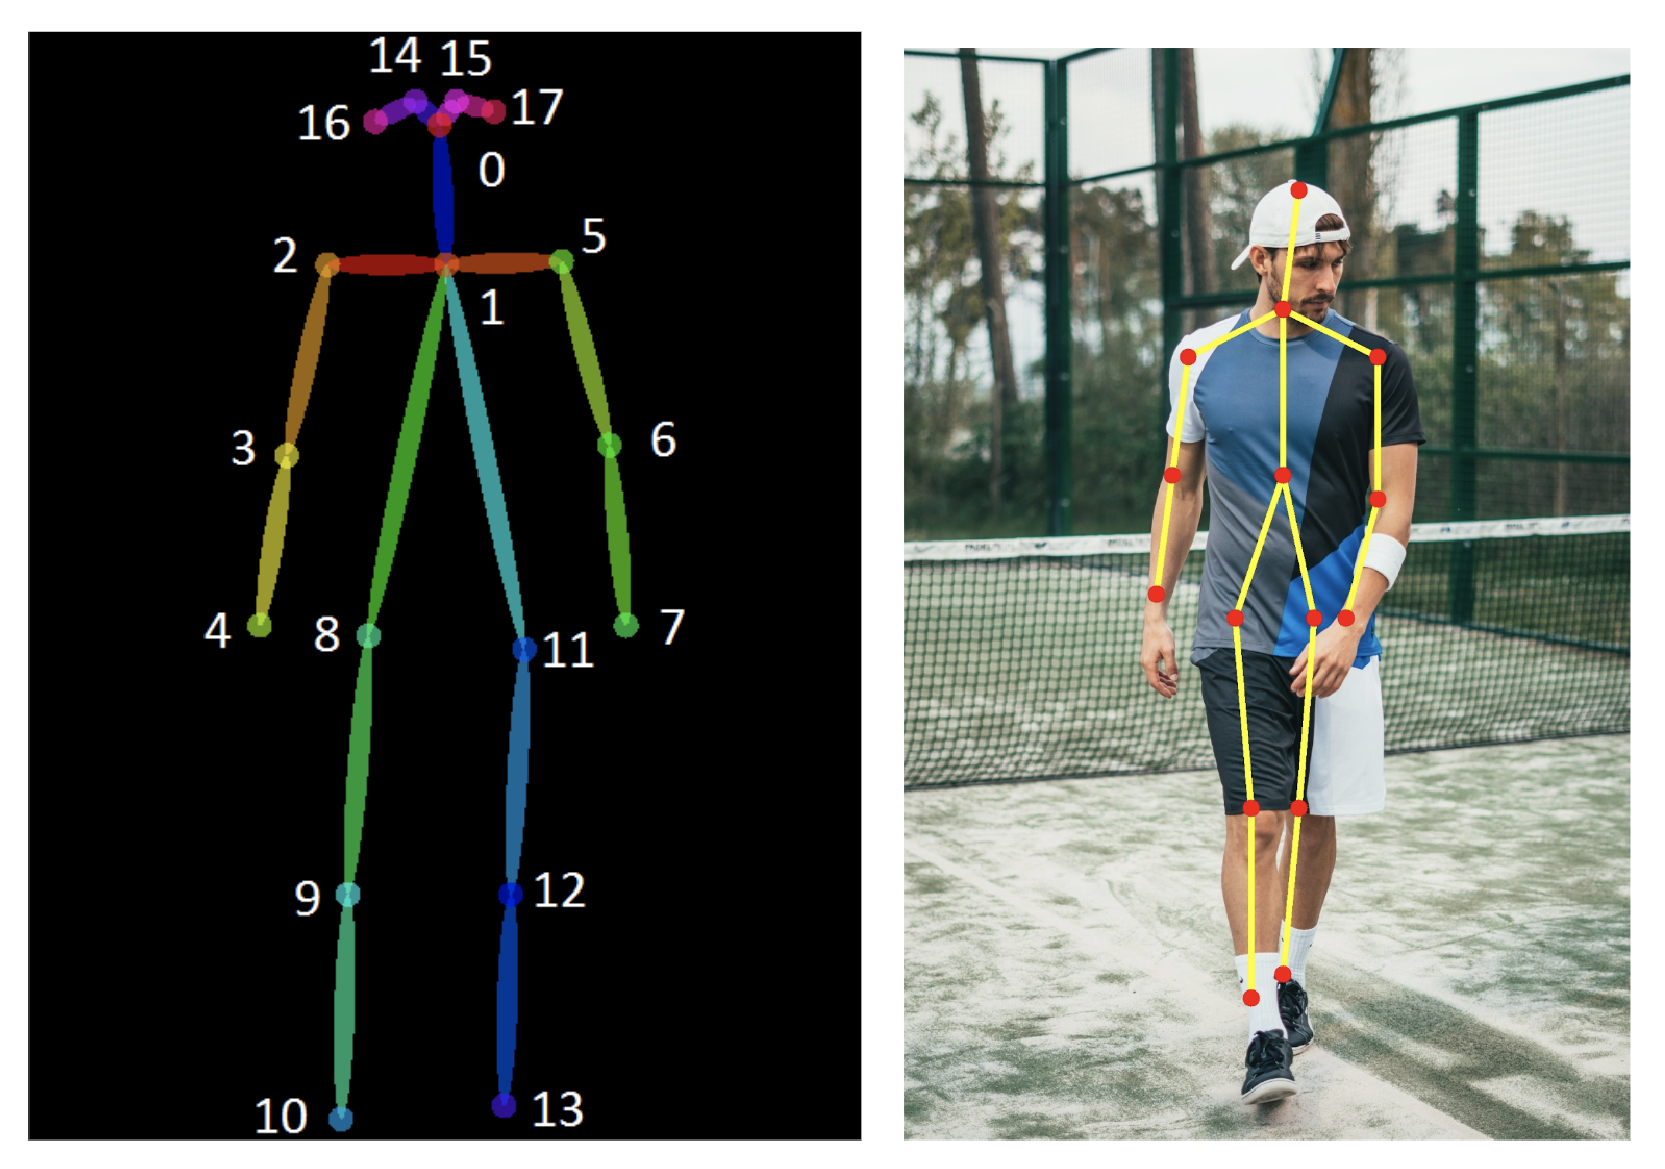
\includegraphics[scale=.3]{pose-estimation}
\caption{Human Pose Estimation Demo}
\end{center}
\end{figure}
An increasing trend in computer vision has driven towards
more efficient models. Recently, Efficient-
Net was released as a scalable ConvNet architecture,
setting benchmark record on ImageNet with a more com-
putationally efficient architecture. 
\section{Problem Statement}

Despite the availability of more performant, efficient layers and architecture's, it has not quite transalated
into fruitful results within human pose estimation, there is still a lack of architectures that
are both accurate and computationally efficient at the same
time. In general, current state-of-the-art architectures are
computationally expensive and highly complex, thus making them hard to replicate, cumbersome to optimize, and
impractical to embed into real-world applications. \par

Minimal and efficient model architectures are coveted for their ability to run on edge devices with minimal hardware requirements.
This also greatly reduces the response times thereby becoming increasingly relevant for real-time applications.
The ability to run real-time is a crucial feature for pose estimation, because often times in most applications it's desirable to obtain the outputs instantly to judge the output.

\section{Objective}

Primary objective is to exploit recent advances in ConvNets and shed some light onto
an improved approach called EfficientPose. The main idea
is to modify OpenPose, a well-known pose estimation model into a family of scalable ConvNets
for high-precision and computationally efficient single-person
pose estimation from 2D images. 
Then we evaluate the EfficientPose model by comparing
it against the original OpenPose model on single-person
HPE. After that, we compare it against the current state-of-
the-art single-person HPE methods on the official MPII
challenge, focusing on accuracy as a function of the number
of parameters. EfficientPose models aim to
elicit high computational efficiency, while bridging the gap
in availability of high-precision HPE networks.

\chapter{Related works}

The world population is the sum of all humans on Earth. As of today, it is estimated to number 7.004 billion by the United States Census Bureau. The USCB estimates that the world population exceeded 7 billion on March 12, 2012. According to a separate estimate by the United Nations Population Fund, it reached this milestone on October 31, 2011.
\begin{table}[h!]
\begin{center}
	\caption{World Population Table} 
\begin{tabular}{|c|c|c|c|}
	
\hline Rank & Country & Population  & Percentage  \\ 
\hline 1 & China & 1,347,350,000 & 19.24\% \\ 
\hline 2 & India & 1,210,193,422  & 17.28\% \\ 
\hline 3 & United States & 313,269,000 & 4.47\% \\ 
\hline 
\end{tabular}
%\caption{World Population Table} 
\end{center}
\end{table}
The world's population is unevenly distributed, with six of Earth's seven continents being permanently inhabited on a large scale. As of 2012, Asia is the most populous continent, with its 4.1 billion inhabitants accounting for over 60\% of the world population. The world's two most-populated countries alone, China and India, constitute about 37\% of the world's population. Africa is the second-most-populated continent, with around 1 billion people, or 15\% of the world's population. Europe's 733 million people make up 11\% of the world's population, while the Latin American and Caribbean regions are home to 589 million (9\%).


\chapter{Design}

In number theory, Fermat's Last Theorem states that no three positive integers a, b, and c can satisfy the equation:
$$
a^{n} + b^{n} = c^{n}
$$ 
for any integer value of n greater than two 

This theorem was first conjectured by Pierre de Fermat in 1637, famously in the margin of a copy of Arithmetica where he claimed he had a proof that was too large to fit in the margin. No successful proof was published until 1995 despite the efforts of countless mathematicians during the 358 intervening years. The unsolved problem stimulated the development of algebraic number theory in the 19th century and the proof of the modularity theorem in the 20th. It is among the most famous theorems in the history of mathematics and prior to its 1995 proof was in the Guinness Book of World Records for "most difficult mathematical problems".

\section{Introduction}
In mathematics, Stirling's approximation (or Stirling's formula) is an approximation for large factorials. It is named after James Stirling.


The formula as typically used in applications is:

$$
\ln (n!) = n \ln n - n  + O(\ln(n))
$$
\section{Design of modules}
In mathematics, Stirling's approximation (or Stirling's formula) is an approximation for large factorials. It is named after James Stirling.

\chapter{Results}

Compiled languages arelanguages typically processed by compilers, though theoretically any language can be compiled or interpreted. The important ones are:
\begin{itemize}
\item Ada
\item C
\item C++
\item Fortran
\item Java
\end{itemize}




\chapter{Conclusion}

An intrusion detection system (IDS) \cite{nist} is a device or software application that monitors network and/or system activities for malicious activities or policy violations and produces reports to a Management Station.


Donald Ervin Knuth \cite{knuth} is a computer scientist and Professor Emeritus at Stanford University. He is the author of the seminal multi-volume work The Art of Computer Programming. Knuth has been called the "father" of the analysis of algorithms


\begin{thebibliography}{1}
\bibitem{nist} K. Scarfone and P. Mell, ``Guide to intrusion detection and prevention systems
(idps),'' \textit{NIST Special Publication}, vol. 800, no. 2007, p. 94, 2007.
\bibitem{knuth} Wikipedia, ``Donald knuth.'' \url{http://en.wikipedia.org/wiki/Donald_Knuth}.
\end{thebibliography}

\begin{appendices}
Test
\end{appendices}


\end{document}
